\section{PIG(12.04.2018)}
Führen Sie folgende Pig Operationen mit Ihren Testdaten (Bags) aus: LOAD,  Dump, Join, Cross, Union, Split

\subsection*{Kurzdarstellung der Aufgabenstellung}
Datensätze in From von .csv Datein in HDFS Ordner Laden und Mittels PIG die im HDFS bereitgestellten Datensätze auswerten. Der grundlegende Umgang mit Daten in PIG als Bestandteil von HADOOP soll durch bereitstellen von Daten in HDFS und das abfragen/analysieren in PIG selbiger geprobt werden.
\subsection*{Lösung}
\begin{itemize}
\item[-] Starten der Oracle 4.9 VM

\item[-] Ändern von Tastaturlayout auf DE mittels Terminaleingabe:
\begin{lstlisting}
setxkbmap -layout de
\end{lstlisting}

\item[-] Anlegen eines eigenes Ordners für die Aufgabenstellung auf der VM:
\begin{lstlisting}
mkdir /usr/tmp/gruppe
\end{lstlisting}

\item[-] Drei Textdateien (artikel, ek\_pos\_1, ek\_pos\_2) in /usr/tmp/gruppe/ mit Testdaten anlegen(\autoref{fig:pig1}):
\begin{figure}[!htb]
        \begin{minipage}{1\textwidth}
                \centering
                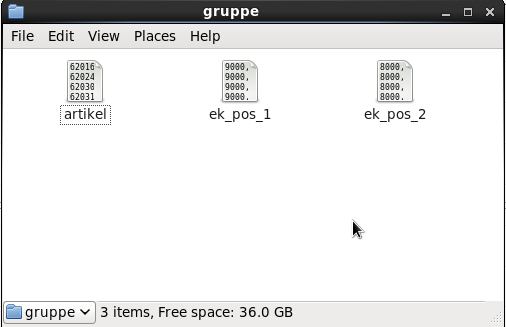
\includegraphics[width=0.90\textwidth]{pics/HDFS_1.png}\par\vspace{0cm}
                \caption{Tabellen}
                \label{fig:pig1}
        \end{minipage}
\end{figure}

\item[-] Über den Termin einen HDFS Ordner fuer die Aufgabenstellung anlegen:
\begin{lstlisting}
hdfs dfs -mkdir hdfs://bigdatalite.localdomain:8020/tmp/gruppe
\end{lstlisting}

\item[-] Zuvor angelegte Textdatei in usr/tmp/gruppe in HDFS Ordner (.../tmp/gruppe) kopieren:
\begin{lstlisting}
hdfs dfs -put /usr/tmp/gruppe/ek_pos_1 hdfs://bigdatalite.localdomain:8020/tmp/gruppe
hdfs dfs -put /usr/tmp/gruppe/ek_pos_2 hdfs://bigdatalite.localdomain:8020/tmp/gruppe
hdfs dfs -put /usr/tmp/gruppe/artikel hdfs://bigdatalite.localdomain:8020/tmp/gruppe
\end{lstlisting}

\item[-] Show files on datastore (printscreen Ergebnis)(\autoref{fig:pig1-1}):
\begin{lstlisting}
hdfs dfs -ls /tmp/gruppe
\end{lstlisting}
\begin{figure}[!htb]
        \begin{minipage}{1\textwidth}
                \centering
                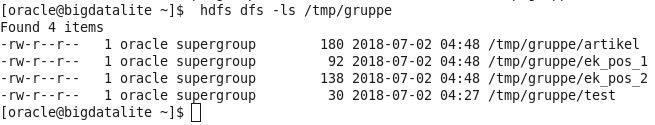
\includegraphics[width=0.90\textwidth]{pics/HDFS_2.png}\par\vspace{0cm}
                \caption{Tabellen im Datastore}
                \label{fig:pig1-1}
        \end{minipage}
\end{figure}

\item[-] Start Pig
\begin{lstlisting}
pig -x mapreduce
\end{lstlisting}

\item[-] pig schließen: 
\begin{lstlisting}
exit the Grunt shell using 'ctrl + d'
\end{lstlisting}

\item[-] Daten aus HDFS Ordner in PIG laden, unter angabe der Spaltennamen und Datentypen:
\begin{lstlisting}
artikel = LOAD 'hdfs://bigdatalite.localdomain:8020/tmp/gruppe/artikel' USING
PigStorage(',') as (art_id:int, art_name:chararray);

ek_pos_1 = LOAD 'hdfs://bigdatalite.localdomain:8020/tmp/gruppe/ek_pos_1'       USING    PigStorage(',') as (kd_id:int, pos:int, art_id:int, menge:int);

ek_pos_2 = LOAD 'hdfs://bigdatalite.localdomain:8020/tmp/gruppe/ek_pos_2'       USING PigStorage(',') as (kd_id:int, pos:int, art_id:int, menge:int);
\end{lstlisting}
\item[-] Ausführen von Abfragen auf den und deren Ausgaben:
\subsubsection*{UNION}
\begin{lstlisting}
ek_positionen = UNION ek_pos_1, ek_pos_2;
dump ek_positionen;
--(8000,1,6202443,2)
--(8000,2,6203175,1)
--(8000,3,6203174,4)
--(8000,4,6203173,2)
--(8000,5,6205923,2)
--(8000,6,6201680,2)
--(9000,1,6203338,2)
--(9000,2,6203207,1)
--(9000,3,6204711,2)
--(9000,4,6203040,2)
\end{lstlisting}

\subsubsection*{JOIN}
\begin{lstlisting}
ek_art_join = JOIN ek_positionen by art_id,artikel by art_id;
dump ek_art_join;
--(8000,6,6201680,2,6201680,ARTIKEL_1)
--(8000,1,6202443,2,6202443,ARTIKEL_2)
--(9000,4,6203040,2,6203040,ARTIKEL_3)
--(8000,4,6203173,2,6203173,ARTIKEL_4)
--(8000,3,6203174,4,6203174,ARTIKEL_5)
--(8000,2,6203175,1,6203175,ARTIKEL_6)
--(9000,2,6203207,1,6203207,ARTIKEL_7)
--(9000,1,6203338,2,6203338,ARTIKEL_8)
--(9000,3,6204711,2,6204711,ARTIKEL_9)
--(8000,5,6205923,2,6205923,ARTIKEL_0)
\end{lstlisting}

\subsubsection*{SPLIT}
\begin{lstlisting}
SPLIT ek_pos_1 into einkauf_1_1 if pos<3, einkauf_1_2 if pos>2;
dump einkauf_1_1;
--(9000,1,6203338,2)
--(9000,2,6203207,1)

dump einkauf_1_2; 
--(9000,3,6204711,2)
--(9000,4,6203040,2)
\end{lstlisting}

\subsubsection*{CROSS}
\begin{lstlisting}
ek_pos_cross = CROSS ek_pos_1, ek_pos_2;
dump ek_pos_cross;
--(9000,4,6203040,2,8000,6,6201680,2)
--(9000,4,6203040,2,8000,5,6205923,2)
--(9000,4,6203040,2,8000,4,6203173,2)
--(9000,4,6203040,2,8000,3,6203174,4)
--(9000,4,6203040,2,8000,2,6203175,1)
--(9000,4,6203040,2,8000,1,6202443,2)
--(9000,3,6204711,2,8000,6,6201680,2)
--(9000,3,6204711,2,8000,5,6205923,2)
--(9000,3,6204711,2,8000,4,6203173,2)
--(9000,3,6204711,2,8000,3,6203174,4)
--(9000,3,6204711,2,8000,2,6203175,1)
--(9000,3,6204711,2,8000,1,6202443,2)
--(9000,2,6203207,1,8000,6,6201680,2)
--(9000,2,6203207,1,8000,5,6205923,2)
--(9000,2,6203207,1,8000,4,6203173,2)
--(9000,2,6203207,1,8000,3,6203174,4)
--(9000,2,6203207,1,8000,2,6203175,1)
--(9000,2,6203207,1,8000,1,6202443,2)
--(9000,1,6203338,2,8000,6,6201680,2)
--(9000,1,6203338,2,8000,5,6205923,2)
--(9000,1,6203338,2,8000,4,6203173,2)
--(9000,1,6203338,2,8000,3,6203174,4)
--(9000,1,6203338,2,8000,2,6203175,1)
--(9000,1,6203338,2,8000,1,6202443,2)
\end{lstlisting}
\end{itemize}
\subsection*{Aufteilung der Aufgaben im Team}
Alle Punkte wurden gemeinsam bearbeitet.
\subsection*{Darstellung der benutzen Werkzeuge und Systeme}
\subsubsection*{Entwurfswerkzeug}
Textdateia(csv)
\subsubsection*{Entwicklungsumgebung}
HDFS
